% -*- mode: latex; -*- mustache tags:  
\documentclass[10pt,twoside,english]{_support/latex/sbabook/sbabook}
\let\wholebook=\relax

\usepackage{import}
\subimport{_support/latex/}{common.tex}

%=================================================================
% Debug packages for page layout and overfull lines
% Remove the showtrims document option before printing
\ifshowtrims
  \usepackage{showframe}
  \usepackage[color=magenta,width=5mm]{_support/latex/overcolored}
\fi


% =================================================================
\title{Learning Object-Oriented Programming, Design and TDD with Pharo}
\author{Stéphane Ducasse}
\series{The Pharo TextBook Collection}

\hypersetup{
  pdftitle = {Learning Object-Oriented Programming, Design and TDD with Pharo},
  pdfauthor = {Stéphane Ducasse},
  pdfkeywords = {Introduction, programming, design, testing, Pharo, Smalltalk}
}


% =================================================================
\begin{document}

% Title page and colophon on verso
\maketitle
\pagestyle{titlingpage}
\thispagestyle{titlingpage} % \pagestyle does not work on the first one…

\cleartoverso
{\small

  Copyright 2017 by Stéphane Ducasse.

  The contents of this book are protected under the Creative Commons
  Attribution-ShareAlike 3.0 Unported license.

  You are \textbf{free}:
  \begin{itemize}
  \item to \textbf{Share}: to copy, distribute and transmit the work,
  \item to \textbf{Remix}: to adapt the work,
  \end{itemize}

  Under the following conditions:
  \begin{description}
  \item[Attribution.] You must attribute the work in the manner specified by the
    author or licensor (but not in any way that suggests that they endorse you
    or your use of the work).
  \item[Share Alike.] If you alter, transform, or build upon this work, you may
    distribute the resulting work only under the same, similar or a compatible
    license.
  \end{description}

  For any reuse or distribution, you must make clear to others the
  license terms of this work. The best way to do this is with a link to
  this web page: \\
  \url{http://creativecommons.org/licenses/by-sa/3.0/}

  Any of the above conditions can be waived if you get permission from
  the copyright holder. Nothing in this license impairs or restricts the
  author's moral rights.

  \begin{center}
    
\includegraphics[width=0.2\textwidth]{_support/latex/sbabook/CreativeCommons-BY-SA.pdf}
  \end{center}

  Your fair dealing and other rights are in no way affected by the
  above. This is a human-readable summary of the Legal Code (the full
  license): \\
  \url{http://creativecommons.org/licenses/by-sa/3.0/legalcode}

  \vfill

  % Publication info would go here (publisher, ISBN, cover design…)
  Layout and typography based on the \textcode{sbabook} \LaTeX{} class by Damien
  Pollet.
}


\frontmatter
\pagestyle{plain}

\tableofcontents*
\clearpage\listoffigures

\mainmatter

\chapter{TinyChat: a fun and small chat client/server}
Pharo allows the definition of a REST server in a couple of lines of code thanks to the Teapot package by zeroflag, which extends the superb HTTP client/server Zinc developed by BetaNine and was given to the community. 
The goal of this chapter is to make you develop, in five small classes, a client/server chat application with a graphical client.
This little adventure will familiarize you with Pharo and show the ease with which Pharo lets you define a REST server.
Developed in a couple of hours, TinyChat has been designed as a pedagogical application. At the end of the chapter, we propose a list of possible improvements. 

TinyChat has been developed by O. Auverlot and S. Ducasse with a lot of fun. 
\section{Objectives and architecture}
We are going to build a chat server and one graphical client as shown in Figure \ref{tinychatclient}. 


\begin{figure}

\begin{center}
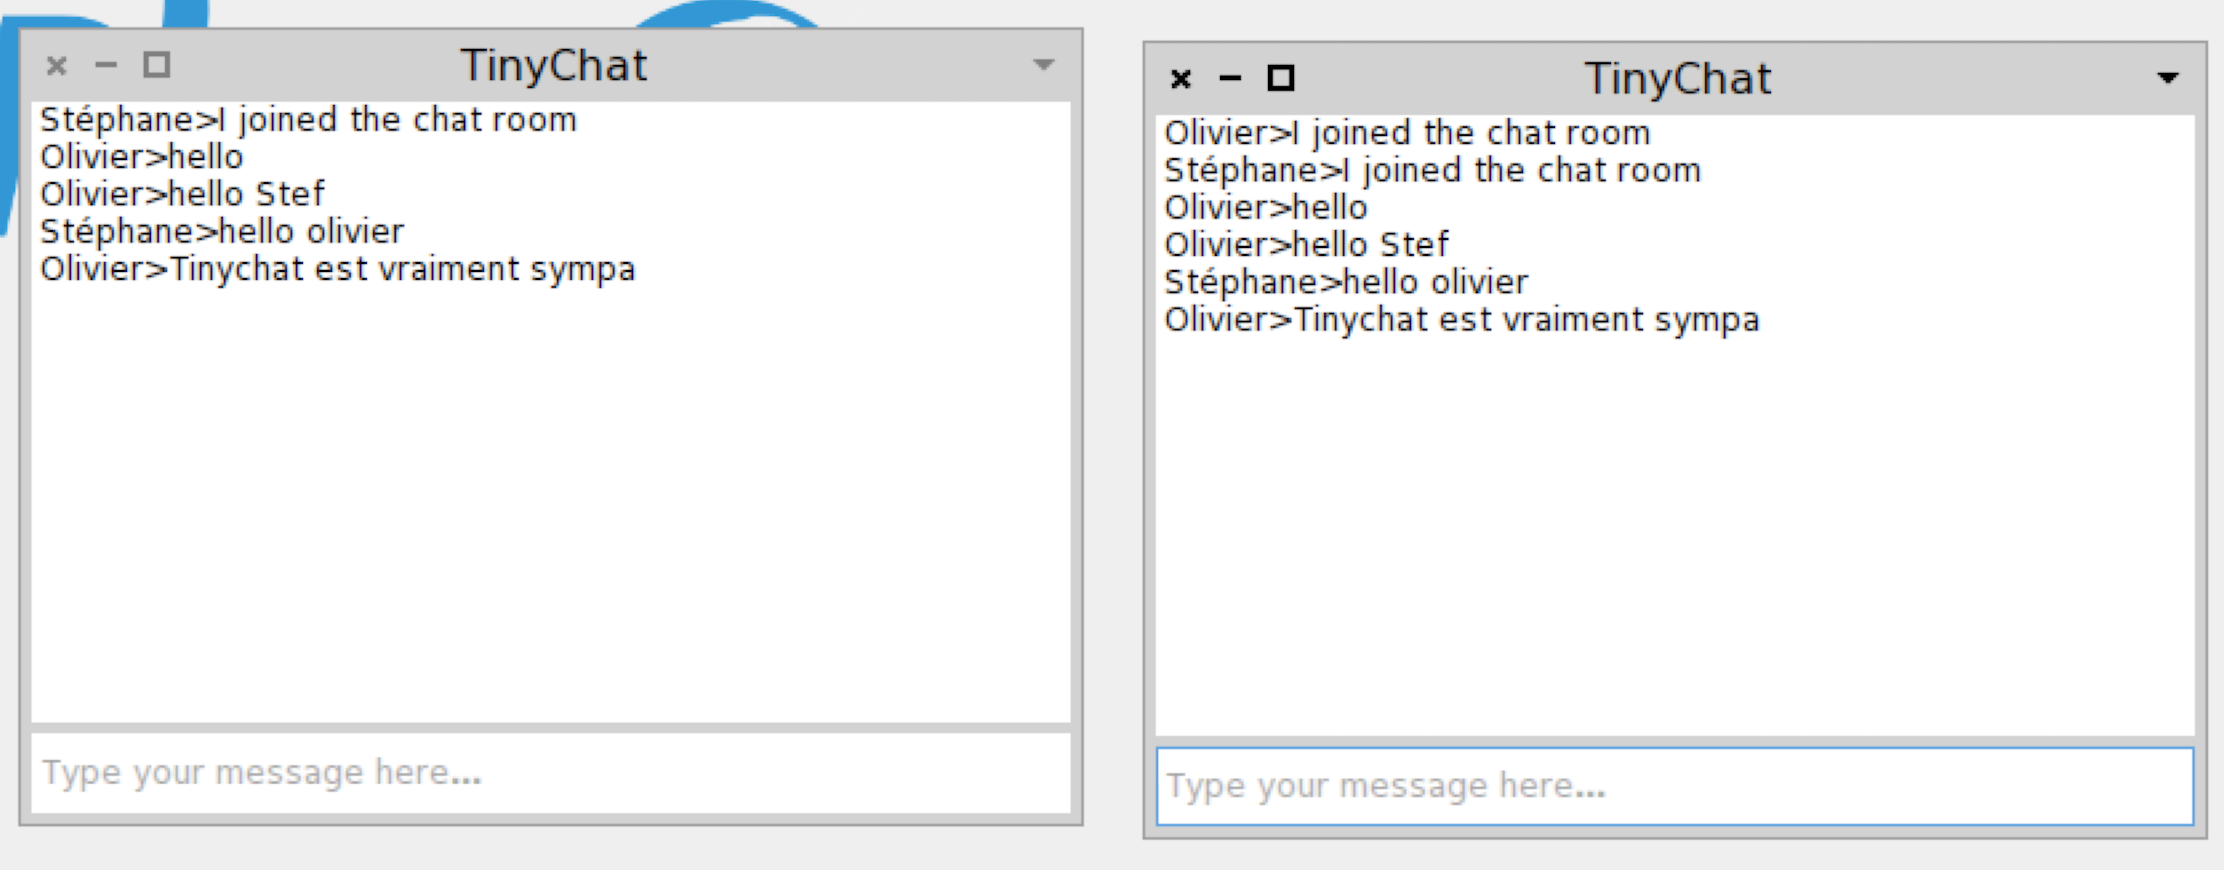
\includegraphics[width=0.8\textwidth]{/Users/ducasse/Workspace/FirstCircle/MyBooks/Bk-Writing/PharoBooks/LearningOOPWithPharoTrans/_result/pdf/Chapters/TinyChat/figures/tinychatclient.png}\caption{Chatting with TinyChat.\label{tinychatclient}}\end{center}
\end{figure}


The communication between the client and the server will be based on HTTP and REST.
In addition to the classes \textcode{TCServer} and \textcode{TinyChat} (the client), we will define three other classes: 
\textcode{TCMessage} which represents exchanged messages (as a future exercise you could extend TinyChat to use 
more structured elements such as JSON or STON (the Pharo object format), \textcode{TCMessageQueue} which stores
messages, and \textcode{TCConsole} the graphical interface.
\section{Loading Teapot}
We can load Teapot using the Configuration Browser, which you can find in the Tools menu item of the main menu.
Select Teapot and click \symbol{34}Install Stable\symbol{34}. Another solution is to use the following script:

\begin{displaycode}{plain}
Gofer it
    smalltalkhubUser: 'zeroflag' project: 'Teapot';
    configuration;
    loadStable.
\end{displaycode}

Now we are ready to start.
\section{Message representation}
A message is a really simple object with a text and sender identifier. 
\subsection{Class TCMessage}
We define the class \textcode{TCMessage} in the package \textcode{TinyChat}.

\begin{displaycode}{plain}
Object subclass: #TCMessage
	instanceVariableNames: 'sender text separator'
	classVariableNames: ''
	category: 'TinyChat'
\end{displaycode}

The instance variables are as follows: 

\begin{itemize}
\item \textcode{sender}: the identifier of the sender,
\item \textcode{text}: the message text, and 
\item \textcode{separator}: a character to separate the sender and the text.
\end{itemize}
\subsection{Accessor creation}
We create the following accessors:

\begin{displaycode}{plain}
TCMessage >> sender
	^ sender

TCMessage >> sender: anObject
	sender := anObject

TCMessage >> text
	^ text

TCMessage >> text: anObject
	text := anObject
\end{displaycode}
\section{Instance initialisation}
Each time an instance is created, its \textcode{initialize} method is invoked. 
We redefine this method to set the separator value to the string \textcode{\textgreater{}}.

\begin{displaycode}{plain}
TCMessage >> initialize
	super initialize.
	separator := '>'.
\end{displaycode}

Now we create a class method named \textcode{from:text:} to instantiate a message (a class method is a method that will be executed on a class and not on an instance of this class):

\begin{displaycode}{plain}
TCMessage class >> from: aSender text: aText
	^ self new sender: aSender; text: aText; yourself
\end{displaycode}

The message \textcode{yourself} returns the message receiver: this way we ensure that the returned object is the new instance and not the value returned by the \textcode{text:} message. This definition is equivalent to the following:

\begin{displaycode}{plain}
TCMessage class >> from: aSender text: aText
	| instance |
	instance := self new.
	instance sender: aSender; text: aText.
	^ instance
\end{displaycode}
\section{Converting a message object into a string}
We add the method \textcode{printOn:} to transform a message object into a character string.
The model we use is sender-separator-text-crlf. Example: 'john\textgreater{}hello !!!'.
The method \textcode{printOn:} is automatically invoked by the method \textcode{printString}. This method is invoked by tools such
as the debugger or object inspector. 

\begin{displaycode}{plain}
TCMessage >> printOn: aStream

	aStream 
		<< self sender; << separator; 
		<< self text; << String crlf
\end{displaycode}
\section{Building a message from a string }
We also define two methods to create a message object from a plain string of the form: \textcode{'olivier\textgreater{}tinychat is cool'}.

First we create the method \textcode{fromString:} filling up the instance variables of an instance. It will be invoked like this: \textcode{TCMessage new fromString: 'olivier\textgreater{}tinychat is cool'}, then the class method \textcode{fromString:} which will first create the instance.

\begin{displaycode}{plain}
TCMessage >> fromString: aString
	"Compose a message from a string of this form 'sender>message'."
	| items |
	items := aString subStrings: separator.
	self sender: items first.
	self text: items second.
\end{displaycode}

You can test the instance method with the following expression \textcode{TCMessage new fromString: 'olivier\textgreater{}tinychat is cool'}.

\begin{displaycode}{plain}
TCMessage class >> fromString: aString
	^ self new 
		fromString: aString;
		yourself
\end{displaycode}

When you execute the following expression \textcode{TCMessage fromString: 'olivier\textgreater{}tinychat is cool'} you should get a message.
We are now ready to work on the server.
\section{Starting with the server}
For the server, we are going to define a class to manage a message queue. This is not really mandatory but it allows
us to separate responsibilities. 
\subsection{Storing messages}
Create the class \textcode{TCMessageQueue} in the package \textit{TinyChat-Server}. 

\begin{displaycode}{plain}
Object subclass: #TCMessageQueue
	instanceVariableNames: 'messages'
	classVariableNames: ''
	category: 'TinyChat-server'
\end{displaycode}

The \textcode{messages} instance variable is an ordered collection whose elements are instances \textcode{TCMessage}.
An \textcode{OrderedCollection} is a collection which dynamically grows when elements are added to it.
We add an instance initialize method so that each new instance gets a proper messages collection.

\begin{displaycode}{plain}
TCMessageQueue >> initialize
	super initialize.
	messages := OrderedCollection new.
\end{displaycode}
\subsection{Basic operations on message list }
We should be able to add, clear the list, and count the number of messages, so we define three methods: \textcode{add:}, \textcode{reset}, and \textcode{size}.

\begin{displaycode}{plain}
TCMessageQueue >> add: aMessage
	messages add: aMessage 

TCMessageQueue >> reset
	messages removeAll

TCMessageQueue >> size
	^ messages size
\end{displaycode}
\subsection{List of messages from a position }
When a client asks the server about the list of the last exchanged messages, it mentions the index of the last
message it knows. The server then answers the list of messages received since this index.

\begin{displaycode}{plain}
TCMessageQueue >> listFrom: aIndex
	^ (aIndex > 0 and: [ aIndex <= messages size]) 
		ifTrue: [ messages copyFrom: aIndex to: messages size ]
		ifFalse: [ #() ]
\end{displaycode}
\subsection{Message formatting}
The server should be able to transfer a list of messages to its client given an index.
We add the possibility to format a list of messages (given an index).
We define the method \textcode{formattedMessagesFrom:} using the formatting of a single message as follows:

\begin{displaycode}{plain}
TCMessageQueue >> formattedMessagesFrom: aMessageNumber
	
	^ String streamContents: [ :formattedMessagesStream |  
		(self listFrom: aMessageNumber) 
			do: [ :m | formattedMessagesStream << m printString ] 
		]
\end{displaycode}

Note how the \textcode{streamContents:} lets us manipulate a stream of characters. 
\section{The Chat server}
The core of the server is based on the Teapot REST framework. It supports the sending and receiving of messages.
In addition this server keeps a list of messages that it communicates to clients. 
\subsection{TCServer class creation}
We create the class \textcode{TCServer} in the \textit{TinyChat-Server} package. 

\begin{displaycode}{plain}
Object subclass: #TCServer
	instanceVariableNames: 'teapotServer messagesQueue'
	classVariableNames: ''
	category: 'TinyChat-Server'
\end{displaycode}

The instance variable \textcode{messagesQueue} represents the list of received and sent messages.
We initialize it like this:

\begin{displaycode}{plain}
TCServer >> initialize
	super initialize.
	messagesQueue := TCMessageQueue new.
\end{displaycode}

The instance variable \textcode{teapotServer} refers to an instance of the Teapot server that we will create using the method \textcode{initializePort:}

\begin{displaycode}{plain}
TCServer >> initializePort: anInteger
	teapotServer := Teapot configure: { 
		#defaultOutput -> #text.
		#port -> anInteger.
		#debugMode -> true
	}.
	teapotServer start.
\end{displaycode}

The HTTP routes are defined in the method \textcode{registerRoutes}. Three operations are defined: 

\begin{itemize}
\item GET \textcode{messages/count}: returns to the client the number of messages received by the server, 
\item GET \textcode{messages/\textless{}id:IsInteger\textgreater{}}: the server returns messages from an index, and
\item POST \textcode{/message/add}: the client sends a new message to the server.
\end{itemize}

\begin{displaycode}{plain}
TCServer >> registerRoutes
	teapotServer
		GET: '/messages/count' -> (Send message: #messageCount to: self);
		GET: '/messages/<id:IsInteger>' -> (Send message: #messagesFrom: to: self);
		POST: '/messages/add' -> (Send message: #addMessage: to: self)
\end{displaycode}

Here we express that the path \textcode{message/count} will execute the message \textcode{messageCount} on the server itself.
The pattern \textcode{\textless{}id:IsInteger\textgreater{}} indicates that the argument should be expressed as number and that it will be converted
into an integer. 

Error handling is managed in the method \textcode{registerErrorHandlers}. Here we see how we can get an instance of the class \textcode{TeaResponse}.

\begin{displaycode}{plain}
TCServer >> registerErrorHandlers
	teapotServer
		exception: KeyNotFound -> (TeaResponse notFound body: 'No such message')
\end{displaycode}

Starting the server is done in the class method \textcode{TCServer class\textgreater{}\textgreater{}startOn:} that gets the TCP port as argument. 

\begin{displaycode}{plain}
TCServer class >> startOn: aPortNumber
	^self new
		initializePort: aPortNumber;
		registerRoutes;
		registerErrorHandlers;
		yourself
\end{displaycode}

We should also offer the possibility to stop the server. The method \textcode{stop} stops the teapot server and empties the message list. 

\begin{displaycode}{plain}
TCServer >> stop
	teapotServer stop.
	messagesQueue reset.
\end{displaycode}

Since there is a chance that you may execute the expression \textcode{TCServer startOn:} multiple times, we define the class method  \textcode{stopAll} which stops all the servers by iterating over all the instances of the class \textcode{TCServer}. 
The method \textcode{TCServer class\textgreater{}\textgreater{}stopAll} stops each server. 

\begin{displaycode}{plain}
TCServer class >> stopAll
	self allInstancesDo: #stop
\end{displaycode}
\section{Server logic}
Now we should define the logic of the server.
We define a method \textcode{addMessage} that extracts the message from the request. It adds a newly created message (instance of class \textcode{TCMessage}) to the list of messages.

\begin{displaycode}{plain}
TCServer >> addMessage: aRequest
	messagesQueue add: (TCMessage from: (aRequest at: #sender) text: (aRequest at: #text)).
\end{displaycode}

The method \textcode{messageCount} gives the number of received messages. 

\begin{displaycode}{plain}
TCServer >> messageCount
	^ messagesQueue size
\end{displaycode}

The method \textcode{messageFrom:} gives the list of messages received by the server since a given index (specified by the client).
The messages returned to the client are a string of characters. This is definitively a point to improve - using string is a poor choice here. 

\begin{displaycode}{plain}
TCServer >> messagesFrom: request
	^ messagesQueue formattedMessagesFrom: (request at: #id)  
\end{displaycode}

Now the server is finished and we can test it. 
First let us begin by starting it:  

\begin{displaycode}{plain}
	TCServer startOn: 8181
\end{displaycode}

Now we can verify that it is running either with a web browser (Figure \ref{running}), or with a Zinc expression as follows: 

\begin{displaycode}{plain}
ZnClient new url: 'http://localhost:8181/messages/count' ; get
\end{displaycode}

Shell lovers can also use the curl command:

\begin{displaycode}{plain}
	curl http://localhost:8181/messages/count
\end{displaycode}


\begin{figure}

\begin{center}
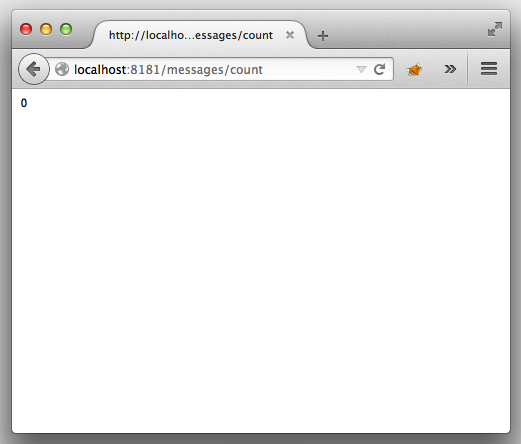
\includegraphics[width=0.8\textwidth]{/Users/ducasse/Workspace/FirstCircle/MyBooks/Bk-Writing/PharoBooks/LearningOOPWithPharoTrans/_result/pdf/Chapters/TinyChat/figures/running.png}\caption{Testing the server.\label{running}}\end{center}
\end{figure}


We can also add a message the following way:

\begin{displaycode}{plain}
ZnClient new 
	url: 'http://localhost:8181/messages/add';
	formAt: 'sender' put: 'olivier';
	formAt: 'text' put: 'Super cool ce tinychat' ; post
\end{displaycode}
\section{The client }
Now we can concentrate on the client part of TinyChat. We decomposed the client into two classes:

\begin{itemize}
\item \textcode{TinyChat} is the class that defines the connection logic (connection, send, and message reception),
\item \textcode{TCConsole} is a class defining the user interface. 
\end{itemize}

The logic of the client is: 

\begin{itemize}
\item During client startup, it asks the server the index of the last received message, 
\item Every two seconds, it requests from the server the messages exchanged since its last connection. To do so, it passes to the server the index of the last message it got. 
\end{itemize}
\subsection{TinyChat class}
We now define the class \textcode{TinyChat} in the package \textcode{TinyChat-client}. 

\begin{displaycode}{plain}
Object subclass: #TinyChat
	instanceVariableNames: 'url login exit messages console lastMessageIndex'
	classVariableNames: ''
	category: 'TinyChat-client'
\end{displaycode}

This class defines the following instance variables:

\begin{itemize}
\item url that contains the server url,
\item login a string identifying the client, 
\item messages is an ordered collection containing the messages read by the client, 
\item lastMessageIndex is the index of the last message read by the client, 
\item exit controls the connection. While exit is false, the client regularly connects to the server to get the unread messages
\item console refers to the graphical console that allows the user to enter and read messages. 
\end{itemize}

We initialize these variables in the following instance \textcode{initialize} method.

\begin{displaycode}{plain}
TinyChat >> initialize
	super initialize.
	exit := false.
	lastMessageIndex := 0.
	messages := OrderedCollection new.
\end{displaycode}
\subsection{HTTP commands}
Now, we define methods to communicate with the server. They are based on the HTTP protocol.
Two methods will format the request. One, which does not take an argument, builds the requests
\textcode{/messages/add} and \textcode{/messages/count}. The other has an argument used to get the message given a position.

\begin{displaycode}{plain}
TinyChat >> command: aPath
	^'{1}{2}' format: { url . aPath }

TinyChat >> command: aPath argument: anArgument
	^'{1}{2}/{3}' format: { url . aPath . anArgument asString }
\end{displaycode}

Now that we have these low-level operations we can define the three HTTP commands of the client as follows:

\begin{displaycode}{plain}
TinyChat >> cmdLastMessageID
	^ self command: '/messages/count'

TinyChat >> cmdNewMessage
	^self command: '/messages/add'

TinyChat >> cmdMessagesFromLastIndexToEnd
	"Returns the server messages from my current last index to the last one on the server."
	^ self command: '/messages' argument: lastMessageIndex
\end{displaycode}

Now we can create commands but we need to emit them. This is what we look at now.
\section{Client operations}
We need to send the commands to the server and to get back information from the server.
We define two methods. The method \textcode{readLastMessageID} returns the index of the last message received from the server.

\begin{displaycode}{plain}
TinyChat >> readLastMessageID
	| id |
	id := (ZnClient new url: self cmdLastMessageID; get) asInteger.
	id = 0 ifTrue: [ id := 1 ].
	^ id
\end{displaycode}

The method \textcode{readMissingMessages} adds the last messages received from the server to the list of messages known by the client. 
This method returns the number of received messages. 

\begin{displaycode}{plain}
TinyChat >> readMissingMessages
	"Gets the new messages that have been posted since the last request."
	| response receivedMessages |
	response := (ZnClient new url: self cmdMessagesFromLastIndexToEnd; get).
	^ response 
		ifNil: [ 0 ]
		ifNotNil: [  
			receivedMessages := response subStrings: (String crlf).
			receivedMessages do: [ :msg | messages add: (TCMessage fromString: msg) ].
			receivedMessages size.
		].
\end{displaycode}

We are now ready to define the refresh behavior of the client via the method \textcode{refreshMessages}.
It uses a light process to read the messages received from the server at a regular interval. 
The delay is set to 2 seconds. (The message \textcode{fork} sent to a block (a lexical closure in Pharo) executes this block in a light process). The logic of this method is to loop as long as the client does not specify to stop via the state of the \textcode{exit} variable. 

The expression \textcode{(Delay forSeconds: 2) wait} suspends the execution of the process in which it is executed for a given number of seconds. 

\begin{displaycode}{plain}
TinyChat >> refreshMessages
	[  
		[ exit ] whileFalse: [  
			(Delay forSeconds: 2) wait.
			lastMessageIndex := lastMessageIndex + (self readMissingMessages).
			console print: messages.
		]
	] fork
\end{displaycode}

The method \textcode{sendNewMessage:} posts the message written by the client to the server. 

\begin{displaycode}{plain}
TinyChat >> sendNewMessage: aMessage
	^ ZnClient new
		url: self cmdNewMessage;
		formAt: 'sender' put:  (aMessage sender);
		formAt: 'text' put: (aMessage text);
		post
\end{displaycode}

This method is used by the method \textcode{send:} that gets the text written by the user. 
The string is converted into an instance of \textcode{TCMessage}. The message is sent and the client updates the index of the last
message it knows, then it prints the message in the graphical interface.

\begin{displaycode}{plain}
TinyChat >> send: aString
	"When we send a message, we push it to the server and in addition we update the local list of posted messages."
	
	| msg |
	msg := TCMessage from: login text: aString.
	self sendNewMessage: msg.
	lastMessageIndex := lastMessageIndex + (self readMissingMessages).
	console print: messages.
\end{displaycode}

We should also handle the server disconnection. We define the method 
 \textcode{disconnect} that sends a message to the client indicating that it is disconnecting and also stops 
 the connecting loop of the server by putting \textcode{exit} to true.

\begin{displaycode}{plain}
TinyChat >> disconnect
	self sendNewMessage: (TCMessage from: login text: 'I exited from the chat room.').
	exit := true
\end{displaycode}
\section{Client connection parameters}
Since the client should contact the server on specific ports, we define a method to 
initialize the connection parameters. We define the class method \textcode{TinyChat class\textgreater{}\textgreater{}connect:port:login:} so that we
can connect the following way to the server: \textcode{TinyChat connect: 'localhost' port: 8080 login: 'username'}

\begin{displaycode}{plain}
TinyChat class >> connect: aHost port: aPort login: aLogin

	^ self new
		host: aHost port: aPort login: aLogin;
		start
\end{displaycode}

\textcode{TinyChat class\textgreater{}\textgreater{}connect:port:login:} uses the method \textcode{host:port:login:}. This method just updates the \textcode{url} instance variable and sets the \textcode{login} as specified.

\begin{displaycode}{plain}
TinyChat >> host: aHost port: aPort login: aLogin
	url := 'http://' , aHost , ':' , aPort asString.
	login := aLogin
\end{displaycode}

Finally we define a method \textcode{start}: which creates a graphical console (that we will define later), tells the server
that there is a new client, and gets the last message received by the server. 
Note that a good evolution would be to decouple the model from its user interface by using notifications. 

\begin{displaycode}{plain}
TinyChat >> start
	console := TCConsole attach: self.
	self sendNewMessage: (TCMessage from: login text: 'I joined the chat room').
	lastMessageIndex := self readLastMessageID.
	self refreshMessages.
\end{displaycode}
\section{User interface}
The user interface is composed of a window with a list and an input field as shown in Figure \ref{tinychatclient}. 

\begin{displaycode}{plain}
ComposableModel subclass: #TCConsole
	instanceVariableNames: 'chat list input'
	classVariableNames: ''
	category: 'TinyChat-client'
\end{displaycode}

Note that the class \textcode{TCConsole} inherits from \textcode{ComposableModel}. This class is the root of the user interface logic classes.
 \textcode{TCConsole} defines the logic of the client interface (i.e. what happens when we enter text in the input field...). Based on the information given in this class, the Spec user interface builder automatically builds the visual representation. 
The \textcode{chat} instance variable is a reference to an instance of the client model \textcode{TinyChat} and requires a setter method (\textcode{chat:}). The \textcode{list} and \textcode{input} instance variables both require an accessor. This is required by the User Interface builder.

\begin{displaycode}{plain}
TCConsole >> input
	^ input

TCConsole >> list
	^ list

TCConsole >> chat: anObject
	chat := anObject
\end{displaycode}

We set the title of the window by defining the method \textcode{title}.

\begin{displaycode}{plain}
TCConsole >> title
	^ 'TinyChat'
\end{displaycode}

Now we should specify the layout of the graphical elements that compose the client.
To do so we define the class method \textcode{TCConsole class\textgreater{}\textgreater{}defaultSpec}. Here we need a column with a list and an input field placed right below. 

\begin{displaycode}{plain}
TCConsole class >> defaultSpec
	<spec: #default>

	^ SpecLayout composed
		newColumn: [ :c | 
			c add: #list; add: #input height: 30 ]; yourself
\end{displaycode}

We should now initialize the widgets that we will use.
The method \textcode{initializeWidgets} specifies the nature and behavior of the graphical components. 
The message \textcode{acceptBlock:} defines the action to be executed then the text is entered in the input field.
Here we send it to the chat model and empty it.

\begin{displaycode}{plain}
TCConsole >> initializeWidgets

	list := ListModel new.
	input := TextInputFieldModel new 
		ghostText: 'Type your message here...';
		enabled: true;
		acceptBlock: [ :string |  
			chat send: string. 
			input text: '' ].
	self focusOrder add: input.
\end{displaycode}

The method \textcode{print} displays the messages received by the client and assigns them to the list contents.

\begin{displaycode}{plain}
TCConsole >> print: aCollectionOfMessages
	list items: (aCollectionOfMessages collect: [  :m |  m printString ])
\end{displaycode}

Note that this method is invoked by the method \textcode{refreshMessages} and that changing all the list elements when we add just one element is rather ugly but ok for now.

Finally we need to define the class method \textcode{TCConsole class\textgreater{}\textgreater{}attach:} that gets the client model as argument.
This method opens the graphical elements and puts in place a mechanism that will close the connection as soon as the client closes the window.
 

\begin{displaycode}{plain}
TCConsole class >> attach: aTinyChat
	| window |
	window := self new chat: aTinyChat.
	window openWithSpec whenClosedDo: [ aTinyChat disconnect ].
	^ window
\end{displaycode}
\section{Now chatting}

\begin{figure}

\begin{center}
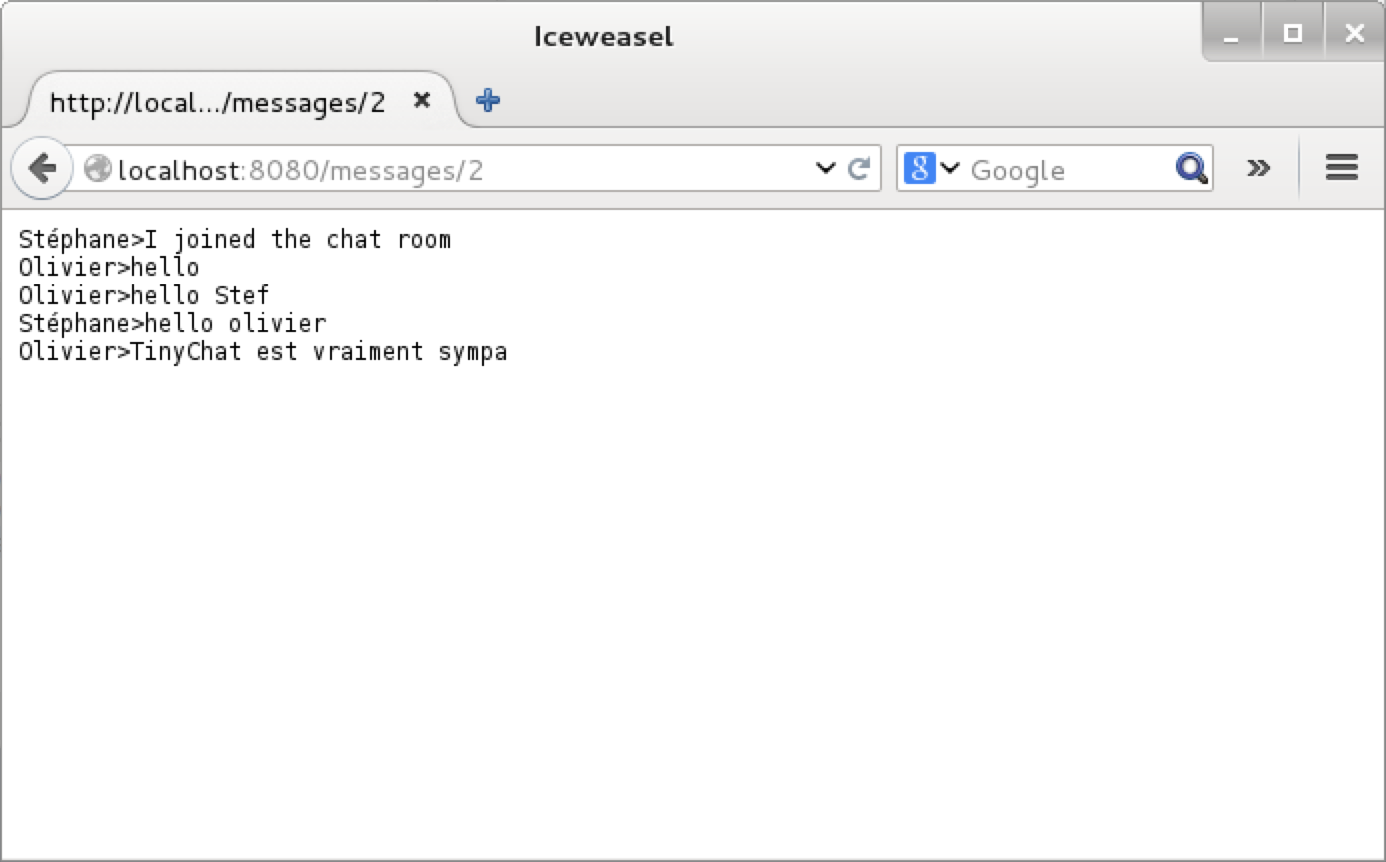
\includegraphics[width=0.6\textwidth]{/Users/ducasse/Workspace/FirstCircle/MyBooks/Bk-Writing/PharoBooks/LearningOOPWithPharoTrans/_result/pdf/Chapters/TinyChat/figures/messages.png}\caption{Server access.\label{messages}}\end{center}
\end{figure}


Now you can chat with your server. The example resets the server and opens two clients.

\begin{displaycode}{plain}
| tco tcs |
TCServer stopAll.
TCServer startOn: 8080.
tco := TinyChat connect: 'localhost' port: 8080 login: 'olivier'.
tco send: 'hello'.
tcs := TinyChat connect: 'localhost' port: 8080 login: 'Stef'.	
tcs send: 'salut olivier'
\end{displaycode}
\section{Conclusion and ideas for future extensions}
We show that creating a REST server is really simple with Teapot. 
TinyChat provides a fun context to explore programming in Pharo and we hope that you like it. 
We designed TinyChat so that it favors extensions and exploration. Here is a list of possible extensions.

\begin{itemize}
\item Using JSON or STON to exchange information and not plain strings.
\item Making sure that the clients can handle a failure of the server.
\item Adding only the necessary messages to the list in the graphical client. 
\item Managing concurrent access in the server message collection (if the server should handle concurrent requests the current implementation is not correct).
\item Managing connection errors. 
\item Getting the list of connected users. 
\item Editing the delay to check for new messages. 
\end{itemize}

There are probably more extensions and we hope that you will have fun exploring some.  
The code of the project is available at  \url{http://www.smalltalkhub.com/#!/~olivierauverlot/TinyChat}.


% lulu requires an empty page at the end. That's why I'm using
% \backmatter here.
\backmatter

% Index would go here
\bibliographystyle{abbrv}
\bibliography{others.bib}
\end{document}
